
\documentclass[tikz,border=2mm]{standalone}
\usepackage[utf8]{inputenc}
\usepackage[T1]{fontenc}
\usepackage{amsmath}
\usepackage{amssymb}
\usetikzlibrary{arrows.meta,positioning,calc,shapes.geometric}
\usepackage{xcolor}

\definecolor{inkNavy}{HTML}{1B2733}
\definecolor{slate}{HTML}{3B4B5C}
\definecolor{paper}{HTML}{FBFAF7}
\definecolor{amber}{HTML}{C97A2B}
\definecolor{teal}{HTML}{2E7D74}
\definecolor{softred}{HTML}{A6402F}
\definecolor{lightgrey}{HTML}{E7E4DD}
\definecolor{midgrey}{HTML}{8B8A85}

\begin{document}
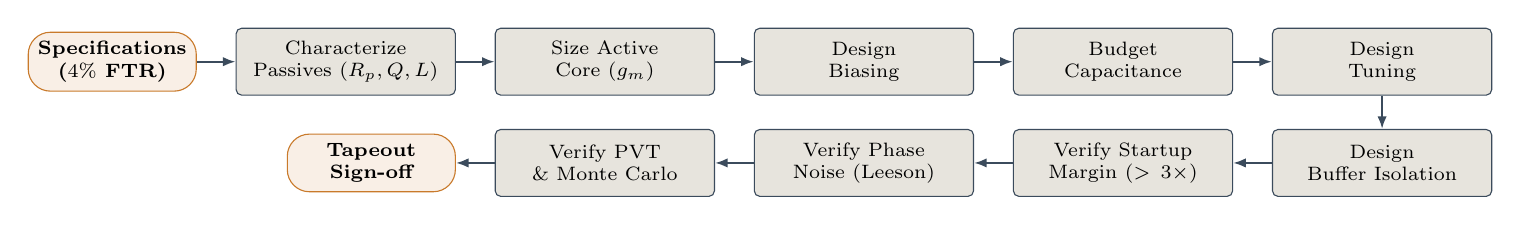
\begin{tikzpicture}[
  node distance=6pt and 14pt,
  box/.style={draw=slate, fill=lightgrey, rounded corners=2pt, text width=2.55cm, align=center, minimum height=0.85cm, font=\scriptsize},
  term/.style={draw=amber, fill=amber!12, rounded corners=8pt, text width=1.9cm, align=center, minimum height=0.7cm, font=\scriptsize\bfseries},
  arr/.style={-{Latex[length=1.6mm]}, slate, thick}
]
\node[term] (spec) {Specifications\\($4\%$\ FTR)};
\node[box, right=of spec] (pass) {Characterize\\Passives ($R_p,Q,L$)};
\node[box, right=of pass] (core) {Size Active\\Core ($g_m$)};
\node[box, right=of core] (bias) {Design\\Biasing};
\node[box, right=of bias] (cap) {Budget\\Capacitance};
\node[box, right=of cap] (tune) {Design\\Tuning};

\node[box, below=12pt of tune] (buf) {Design\\Buffer Isolation};
\node[box, left=of buf] (start) {Verify Startup\\Margin ($>3\times$)};
\node[box, left=of start] (pn) {Verify Phase\\Noise (Leeson)};
\node[box, left=of pn] (pvt) {Verify PVT\\\& Monte Carlo};
\node[term, left=of pvt] (fin) {Tapeout\\Sign-off};

\draw[arr] (spec)--(pass); \draw[arr] (pass)--(core); \draw[arr] (core)--(bias);
\draw[arr] (bias)--(cap); \draw[arr] (cap)--(tune); \draw[arr] (tune)--(buf);
\draw[arr] (buf)--(start); \draw[arr] (start)--(pn); \draw[arr] (pn)--(pvt);
\draw[arr] (pvt)--(fin);
\end{tikzpicture}
\end{document}